\section{System Overview}
\label{sec-system}

\begin{figure}
\centering
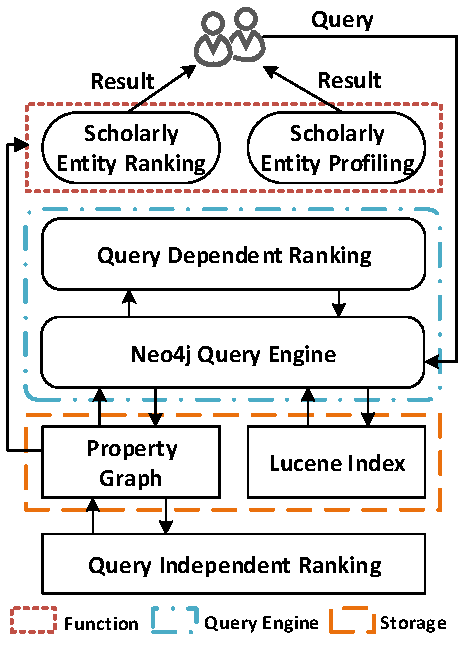
\includegraphics[width=\columnwidth]{systemFrame.pdf}
\caption{system framework}
\label{fig:frame}
\end{figure}


\begin{figure}
\centering
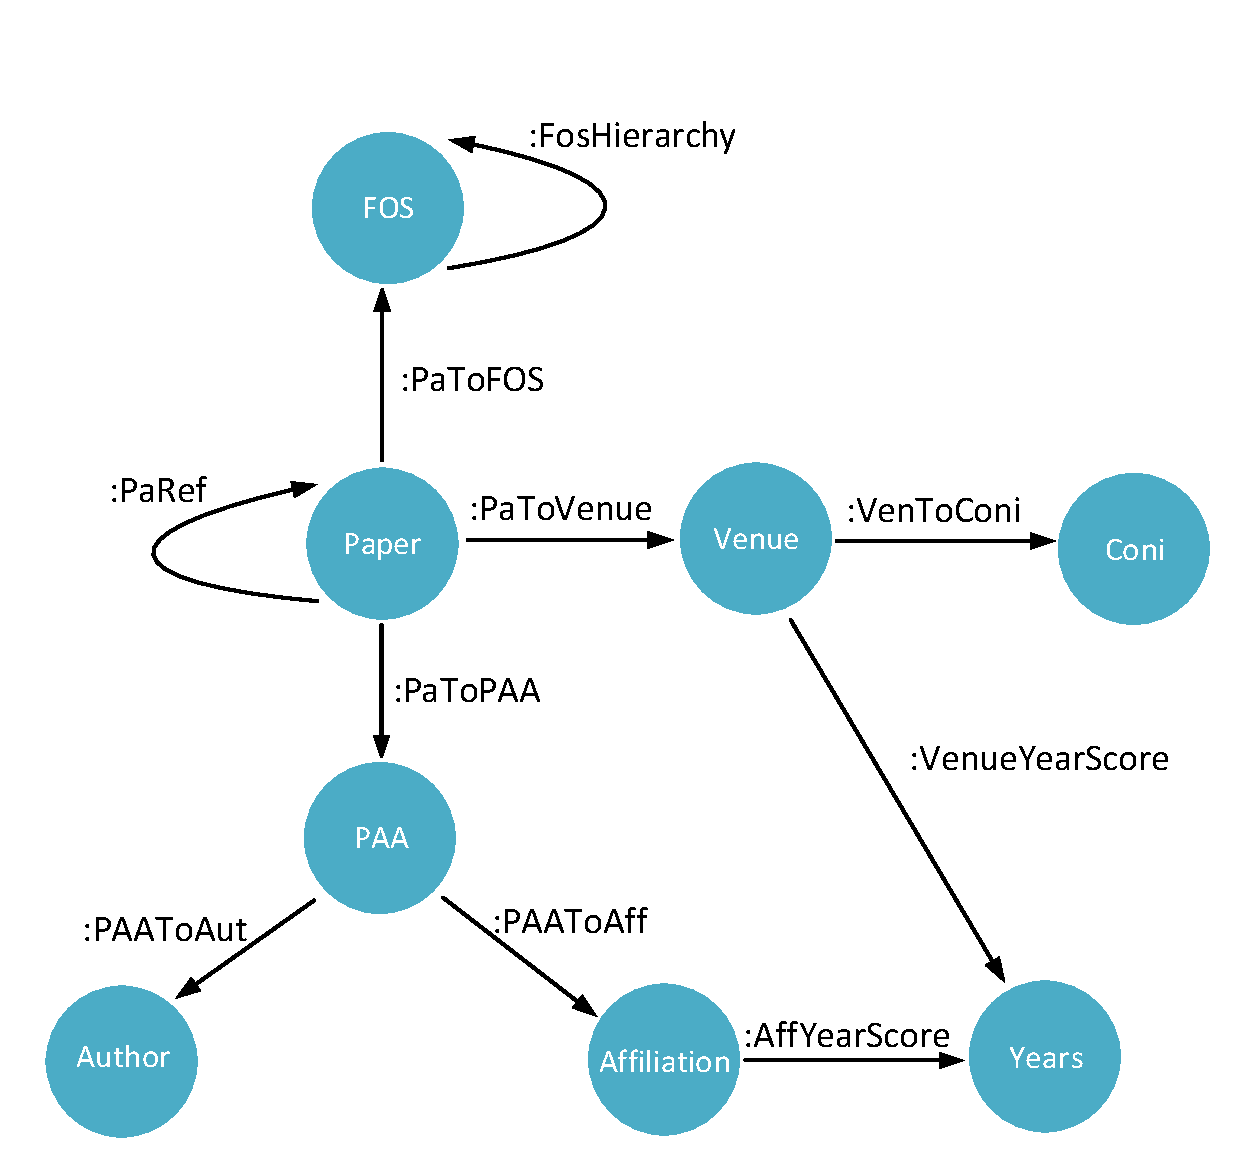
\includegraphics[width=\columnwidth]{neo4jSchema.pdf}
\caption{Neo4j schema design}
\label{fig:schema}
\end{figure}

\begin{figure*}[tp]
\centering
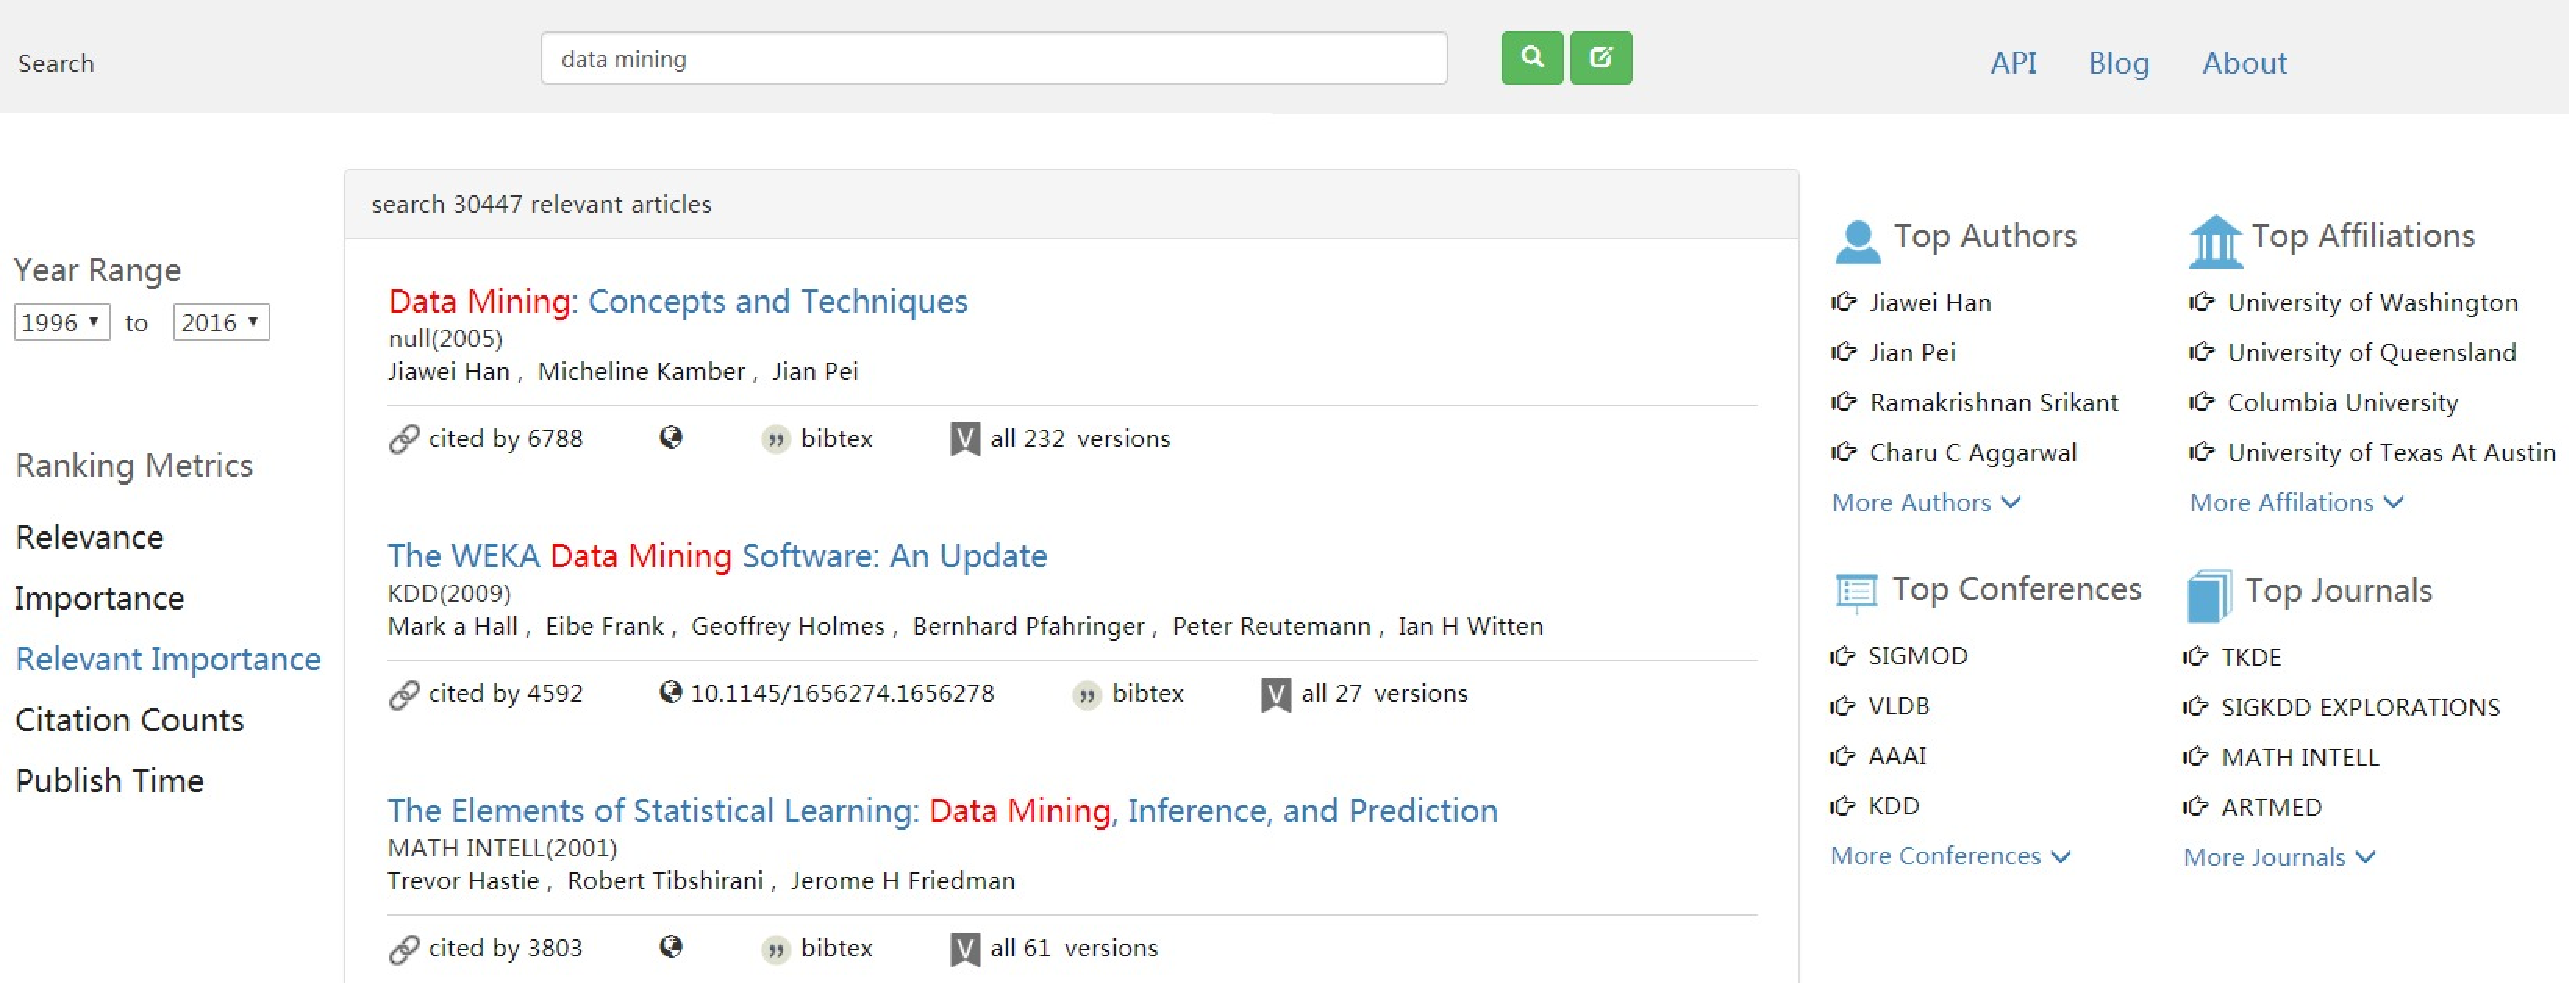
\includegraphics[width=\textwidth]{searchKeywords.pdf}
\caption{search keywords : graph database}
\label{fig: search keywords}
\end{figure*}

\par
We mainly use Microsoft Academic Graph(MAG) to build \oursystem \cite{sinha2015overview}. It contains about 126 million scientific publication records, 529 million citation relationship and other scholarly activities information. Fig. \ref{fig:frame} shows the framework of our system, which consists of three main components, \emph{Storage, Query Engine} and \emph{Visualizer} respectively. Based on the framework, we then present a set of web-based scenarios using RESTful APIs.
% 126909021 paper  114698044 articles 529 million 

\subsection{System Framework}
%Data source. currently storage solution, shortage, why graph database. storage contents

\subsubsection{Storage}
\par
%We mainly use Microsoft Academic Graph(MAG) to build \oursystem \cite{sinha2015overview}. It contains scholarly information such as author, article, venue, affiliation, field of study as well as other information. Aminer, CiteSeerx and Semantic Scholar use relational database system such as Mysql to store and manage the xxx. 


\par
Scholarly data highly connected by reference relationship between articles and constructs a huge heterogeneous graph. Aminer, CiterSeerx and Semantic Scholar use RDBMS such as Mysql to store and manage scholarly data. While Acemap apply Spark to operate massive memory data and Microsoft Academic use Azure to store those huge data. Take RDBMS as an example, complex joins and self-joins will incur obviously performance bottleneck when the scholarly dataset becomes more inter-related. A comparison of the performance of querying the cited articles of an article using RDBMS(Mysql) and graph database(Neo4j) is given in table 1. Furthermore, our heterogeneous entities ranking algorithm, a type of Time-Weighted PageRank, assesses the importance of nodes in a heterogeneous graph. Thus, it utilizes graph database to manage and operate heterogeneous scholarly data.
% scholarly data source, currently solution, why graph database. 

\par 
The component of storage consists of property graph and transaction. Heterogeneous academic data is stored as property graph model which possesses nodes and relationships, and we use transaction to ensure the predictability of relationship-based queries.
% storage

\par
In order to manage effectively and query efficiently with Neo4j, we design a graph schema mainly based on two principles. (1) Nodes for things and relationships for structure. (2) We take into consideration of the query ability of the graph schema and adopt time and space trade-offs. Thus, we model scholarly data as a huge heterogeneous graph, shown in Fig. \ref{fig:schema}, which contains more than one billion nodes and over two billion relationships.


-------------------- original version --------------------  \\

The component of storage consists of property graph and transaction. Heterogeneous academic data is stored as property graph model which possesses nodes and relationships, and we use transaction to ensure the predictability of relationship-based queries.

We apply a popular graph database Neo4j \cite{Neo4j} to manage and operate massive scholarly data based on the following reasons. First, scholarly data is naturally structured data connected by the reference relationship. At the same time, graph database has great performance implementation handling connections. Second, Neo4j is provided with highly performant read and write scalability thanks to native graph storage and processing. Thus, it works well in managing scholarly data and searching subgraphs.

\par
In order to manage effectively and query efficiently with Neo4j, we design a graph schema mainly based on two principles. (1) Nodes for things and relationships for structure. (2) We take into consideration of the query ability of the graph schema and adopt specific trade-offs. Thus, we model academic data as a huge heterogeneous graph, shown in Fig. \ref{fig:schema}, which contains more than one billion nodes and over two billion relationships.



\par
The graph schema contains seven type of entities: author, affiliation, field of study, paper, venue(journal and conferences \itshape e.g., \upshape KDD, ICDE ), conference instance (\itshape e.g., \upshape KDD 2019, ICDE 2019), years. In order to query efficiently, we introduce an additional node PAA to represent the paper-author-affiliation n-ary relationships. Intuitively, a paper get published in a journal/conference by the author means the edges among paper, author and venue node.

\par
By employing ranking model as stated in section 2, we derive affiliation, author, venue and article ranking score using incremental computation \cite{ma2018query}. And those score is described as a property in the graph schema. In fact, we can apply any algorithms to rank scholarly entities in the graph schema.


\subsubsection{Query Engine}
Query engine is the main component that is responsible for retrieving scholarly data from Neo4j. It consists of lucene index, query optimization, Neo4j query engine and ranking algorithm. To query efficiently, we employing lucene index in property of paper title, author name and distributed representation of words. Moreover, we can load a part of index into main-memory to speed up a wide query functions.
Query optimization aims to reduce cardinality of work in the progress to generate a new query plan. Moreover, Neo4j query engine executes the query plan to perform efficient data retrieval. The ranking algorithm is responsible for ranking the results according to SARank, relevance ranking,  \itshape ect. \upshape

%why we need index. index is important for xxx
%what we indexed?
%1. title after using stop word in desk.
%2. vector, word representation
%Query Optimizer and
%Neo4j Query Engine
%Ranking Algorithm
%relevance, ranking results.

\subsubsection{Visualizer}
With all the technical details of managing and querying scholarly data in the system back-end, the ranking system takes users queries through user interfaces, dispatches them to the query engine, and receives the answers back to visualize. The next section presents some scenarios to demonstrate the front-end.


\subsection{System Demonstration}
Fig. \ref{fig: search keywords}, search keywords: given a search ``graph database". It has four major areas: (1) Area 1, the top of the picture, where users can search keywords, authors and affiliations. (2) Area 2 presents relevant papers about the keywords, which is in the center of the picture. (3) At left of the picture is Area 3, we can choose different ranking type, such as SARank, relevance ranking, most citation and time ranking. (4) Top-k prestige authors, influential affiliations, famous journals/conferences is show in Area 4, which is at the right of the picture.


